\chapter{Introduction}
\label{cha:intro}


\section{Thesis Statement}
\label{sec:thesisstatement}
FaceX is a lightweight, flexible and scalable engine that can be used to generate a variety of high-quality images with diversity of facial expressions and shapes. 


\section{Introduction}
\label{sec:problemstatement}
% Put your introduction here. You could use \textbackslash fix\{ABCDEFG.\} to
% leave your comments, see the box at the left side. \fix{You have to rewrite your
% thesis!!!}

In the last few decades, facial expression analysis (FEA) is a challenging task of computer vision and has attracted the interest of more and more researchers. Facial expression has been proven to play important role in understanding human emotion \citep{Mehrabian_Russell_1974}. Because facial expression is the response of a person's mental state to external stimuli \citep{Cabanac_2002}. And \citeauthor{ekmanArgumentBasicEmotions1992} classifies human emotions into seven basic categories: Happy, Sad, Surprise, Anger, Disgust, Fear and Neutral based on cross-culture study. In recent years, Compound Emtions(CEs)~\citep{duCompoundFacialExpressions2014} and Micro Expressions(MEs)~\citep{ekmanDarwinDeceptionFacial2006} have also been explored, but achievements are not rich.

With the development of artificial intelligence, especially machine learning (ML), people benefit from artificial intelligence agents adjusting their response according to their emotional state \citep{adolphsInvestigatingEmotionsFunctional2018}. In this regard, 
there are braod facial expression applications in different domains like Human-Centred Computing(Hcc) \citep{cowieEmotionRecognitionHumancomputer2001}, augmented reality (AR) \citep{chenAugmentedRealitybasedSelffacial2015}, virtual reality (VR) \citep{bekeleUnderstandingHowAdolescents2013}, automatic driving \citep{jabonFacialExpressionAnalysis2011}, and gaming \citep{lankesFacialExpressionsGame2008}. 

Various types of data can feed the FEA systems. In computer vision, facial images are the mainstream input data type. In addition, electromyography (EMG), electrocardiographic(ECG) and other related physical or chemical signal can be used as input data or auxiliary data as well \citep{jerrittaPhysiologicalSignalsBased2011}. This thesis focus on using facial images taken by sensor to detect expression and feeling of people. Because facial images contain sufficient non-verbal information for FEA \citep{huangFacialExpressionRecognition2019}. 

We briefly review the development of FEA in computer vision, most of FEA techniques can be defined as either traditional methods or learning-based methods \citep{huangFacialExpressionRecognition2019}.

\textbf{Traditional methods} involves various hand-craft features. Those approaches need to design appropriate feature extraction and choose different classifier for different dataset. Lots of conventional FEA technicals can be summarized into three main steps: preprocessing, feature extraction, facial expression classification. Preprocessing aims to reduce irrelevant redundant information and improve the ability to recognize related information. Image noise reduction, face detection and alignment and image enhancement are popular preprocessing methods. As for feature extraction, Local Binary Pattern(LBP) \citep{ahonenFaceRecognitionLocal2004}, Optical Flow \citep{hornDeterminingOpticalFlow1981}, Gabor feature \citep{lyonsCodingFacialExpressions1998},and etc. are commonly used in FEA. Another important aspect of traditional FEA methods is selecting classifier to predict facial expression. Support Vector Machine (SVM), k-Nearest Neighbours (kNN), Adaptive Boosting (Adaboost) and etc. classical ML classifier are widely deployed in FEA system. 

On the other hand,\textbf{Learning-based methods} especially for Deep-Learning (DL) have gradually become mainstream due to the great-leap-forward development of computing resources and datasets. Although the DL method outperforms and is more robust than traditional methods because it reduces the dependence on image preprocessing and hand-craft features, DL requires a huge volume of high-quality data for training compared to traditional methods. According to \citeauthor{rohSurveyDataCollection2019}, appropriate high-quality representative training data has become the bottleneck of DL. Regardless of the model, computing resources are no longer the main limitation of the end performance. Data augmentaion can alleviate the problem of insufficient data in some extent, but it is limited to the dataset itself \citep{shortenSurveyImageData2019a}. Therefore, we hope to solve this problem with pure synthetic methods. Despite the pure synthetic method greatly increases the diversity of the dataset, how to shrink the domain gap between the synthetic data set and the real data distribution is still the biggest challenge.

In this work, in order to tackle the problem of synthetic facial expression data we need to evaluates some publicly available datasets for FEA. \citep{khanSurveyAnalysisHuman2020} summarize that the facial expression dataset can be divided into video dataset and image dataset. Most public datasets only contain less than 10k images like DISFA \citep{mavadatiDISFASpontaneousFacial2013} , and some dataset less 200+ images like JAFFE \citep{lyonsCodingFacialExpressions2020}. Only a few data sets contain more than 1 million images like EmotioNet \citep{benitez-quirozEmotioNetAccurateRealTime2016a}. However, Some datasets capture a large number of images from the Internet, others are poor resolution, or the distribution of expressions is uneven. Therefore, We propose a facial expression data synthesis engine based on 3D morphable face model. This engine can synthesize a large number of labeled data with different shape, various expressions, and flexible poses. Figure \ref{fig:overview} show an overview of our engine.

\begin{figure}
    \centering
    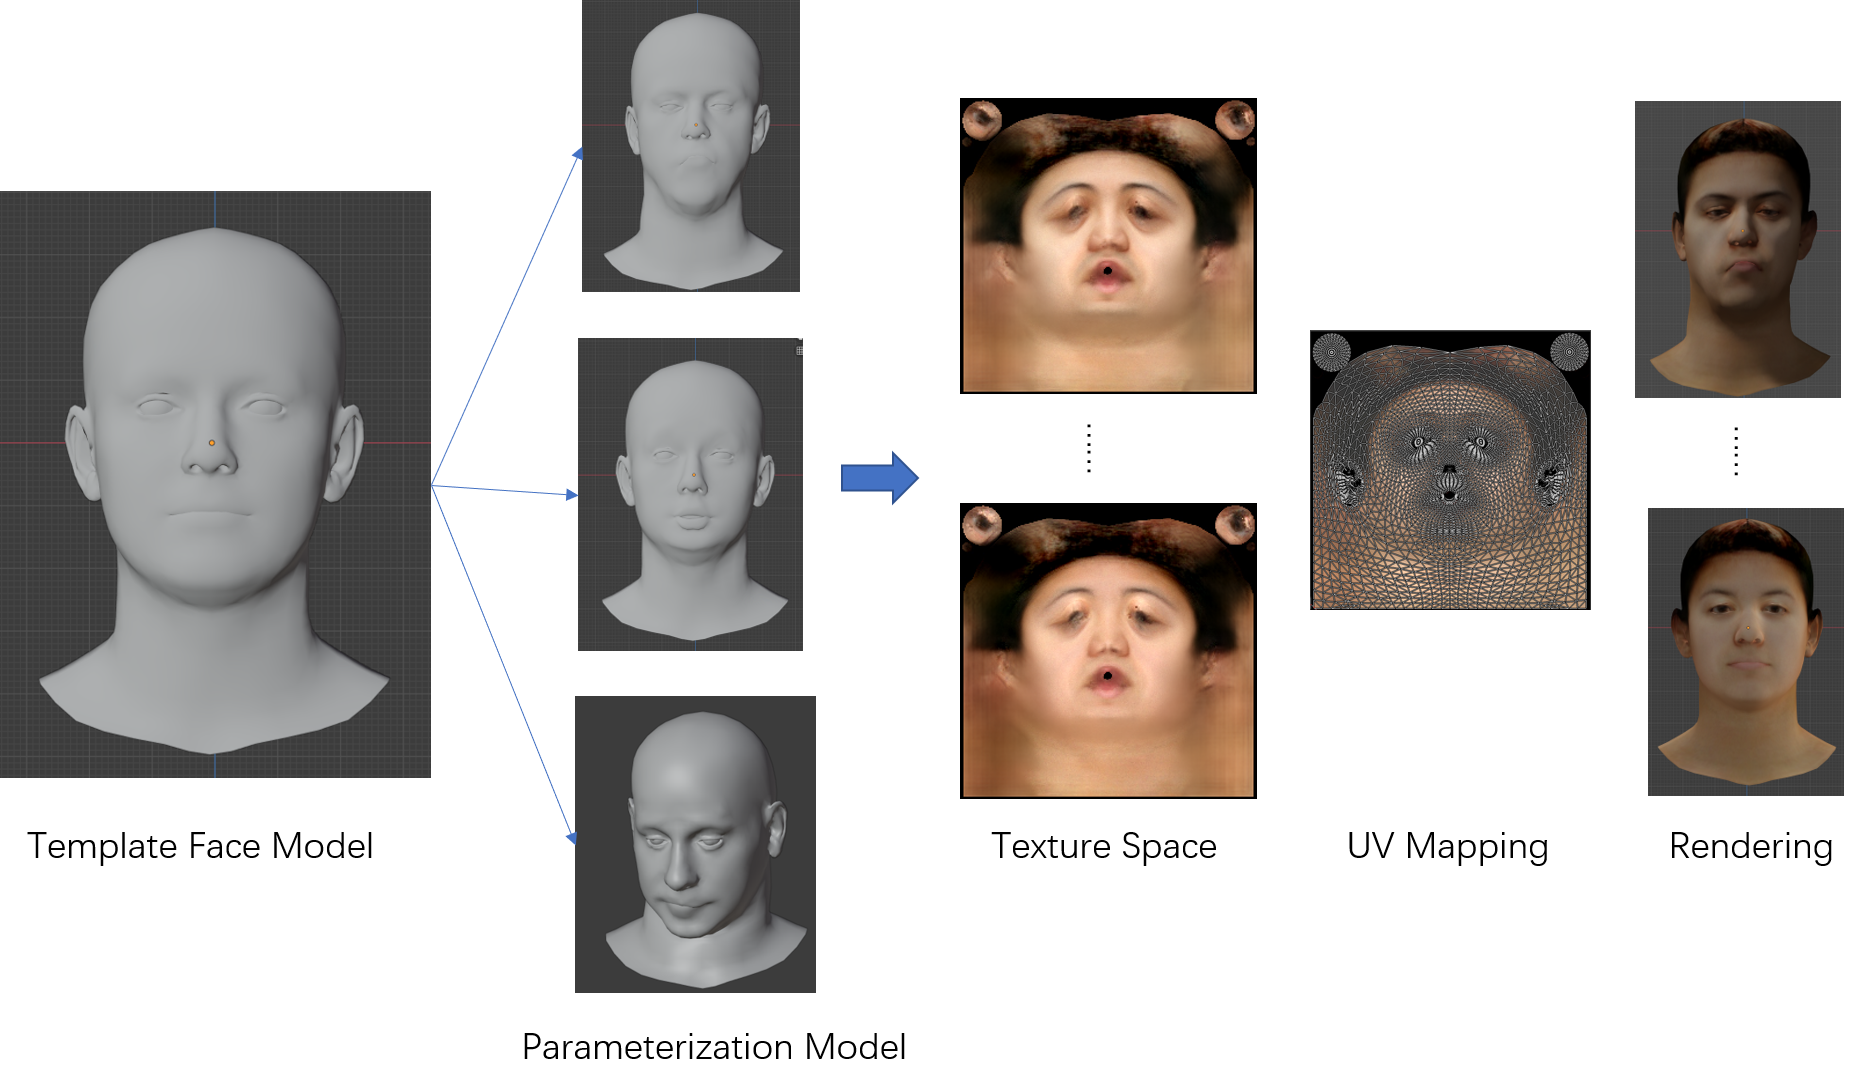
\includegraphics[width=\textwidth]{./figs/overview.png}
    \caption{Our proposed engine. We are able to generate large-scale facial expression data sets for training deep neural networks. We set the initial face model with different shape, expression and pose parameters, and sample different materials from the texture space to map to the model. Finally render under different lighting parameters.}
    \label{fig:overview}
\end{figure}


%%%%%%%%%%%%%%%%%%%%%%%%%%%%%%%%%%%%%%%%%%%%%%%%%%%%%%%%%%%%%%%%

In summary, the contributions of this thesis are as following:

\begin{itemize}
    \item Briefly summarize the development of FEA recently, and try to use synthetic data to solve the DL data bottleneck. (Section \ref{sec:problemstatement}, Chapter \ref{cha:background})
    \item Build a complete synthetic data engine, including various face shape, expression, pose and texture. (Chapter \ref{cha:design})
    \item Measure the performance of DL method on synthetic dataset. (Chapter \ref{cha:methodology})
    \item Discusse the potential problems of the synthetic data, and explain  possible improvement. (Chapter \ref{cha:conc})
\end{itemize}

\section{Thesis Outline}
\label{sec:outline}
The rest of thesis is organized from motivation to building of synthetic facial expression images.

Chapter~\ref{cha:background} introduces some details of the traditional FEA method and Deep Learning-based method, and reviews the existing FE datasets, as well as 3D Morphable Face Models (3DMM) that can be used for data synthesis.

Chapter~\ref{cha:design} describes the pipeline of the data synthesis engine.

Chapter~\ref{cha:methodology} is the detial of experimental design  and synthetic dataset.

Chapter~\ref{cha:result} and Chapter~\ref{cha:conc} are the results of experiments and related analytic demonstration.


